\section{Digital histopathological images}

\glsreset{WSI}
\glsreset{ROI}

Digital histopathology represents a significant advancement in
medical imaging, where traditional glass slides containing tissue
samples are digitized using specialized scanning devices. This
transformation has revolutionized the field of pathology by enabling
remote diagnosis, computer-aided analysis, and digital archiving of
tissue samples \cite{AmgadEtAl2019}. This process has evolved
significantly over the past few decades, as shown in Figure
\ref{fig:histology_evolution}.

\begin{figure}[h]
  \centering
  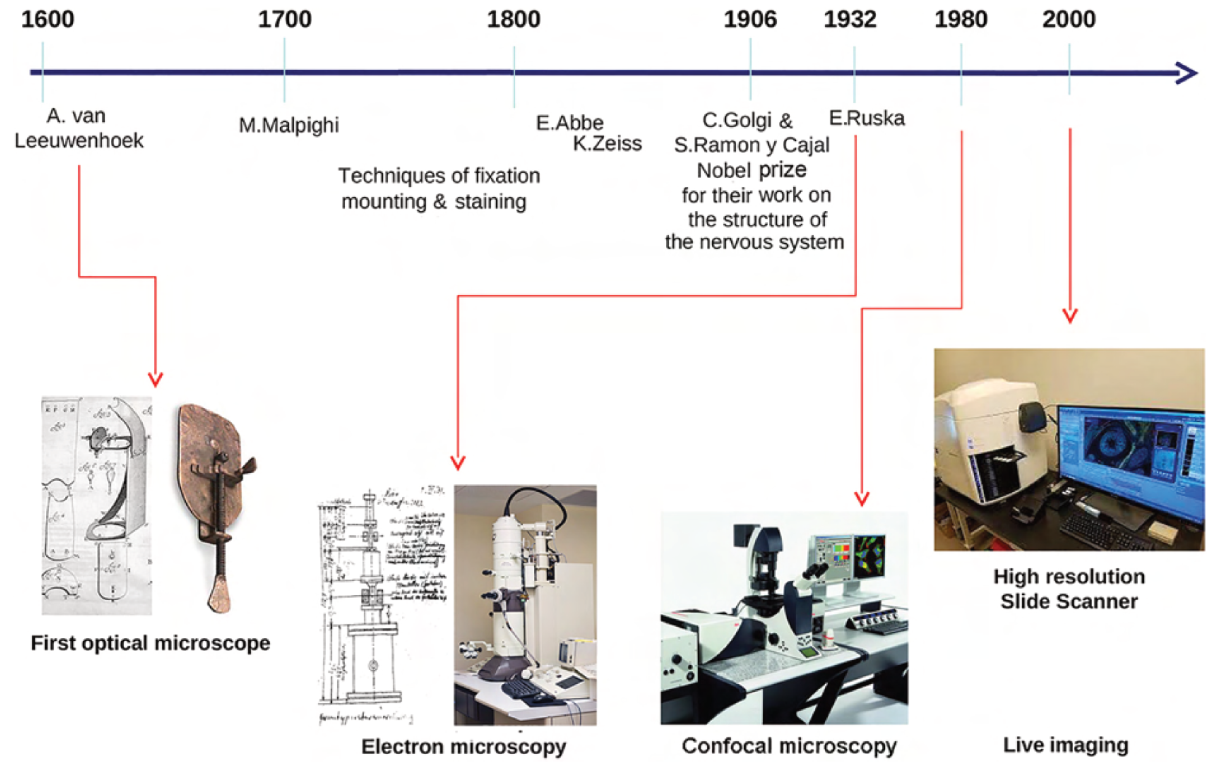
\includegraphics[width=0.65\textwidth]{Cap2/Figures/histology_evolution.png}
  \caption{Histology evolution timeline. (Image from \cite{MazzariniEtAl2021}).}
  \label{fig:histology_evolution}
\end{figure}

\subsection{Whole Slide Imaging (WSI)}

\gls{WSI} is the process of digitizing entire glass
slides at high resolution, creating a digital representation that can
be viewed, analyzed, and shared electronically. Modern \gls{WSI} scanners
use sophisticated optical systems that capture multiple fields of
view at high magnification, which are then stitched together to
create a seamless digital image \cite{DingyiEtAl2025}. These systems incorporate
high-resolution objectives with magnifications ranging from 20x to
40x, precise motorized stages for accurate slide positioning,
automated focus systems to maintain image quality, and high-quality
cameras equipped with large sensor arrays. The resulting digital
slides can reach sizes of several gigabytes, containing billions of
pixels that capture the microscopic details of tissue samples
\cite{DingyiEtAl2025}. Figure \ref{fig:wsi} shows a whole slide
imaging system by Omnyx for slide digitization and a comprehensive
digital pathology interface from Omnyx designed to streamline
pathologists' diagnostic workflow \cite{FarahaniEtAl2015}.

\begin{figure}[h]
  \centering
  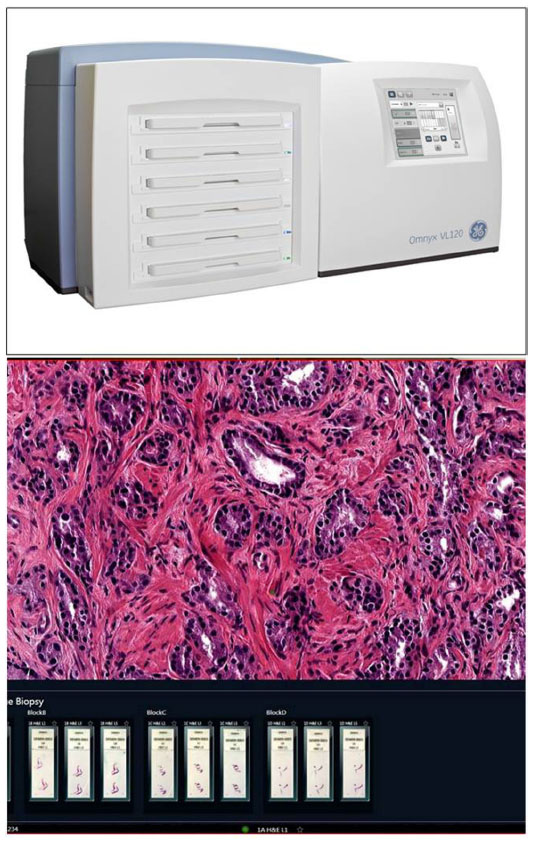
\includegraphics[width=0.5\textwidth]{Cap2/Figures/hist_scanner.jpg}
  \caption{(Above) Whole slide imaging system by Omnyx for slide
    digitization. (Below) Comprehensive digital pathology interface
    from Omnyx designed to streamline pathologists' diagnostic
  workflow. (From \cite{FarahaniEtAl2015}).}
  \label{fig:wsi}
\end{figure}

\subsection{Regions of Interest (ROI)}

In digital histopathology, \glspl{ROI} are specific areas within a
whole slide image that contain diagnostically relevant information.
These regions can be manually annotated by pathologists,
automatically detected using computer vision algorithms, or defined
based on specific tissue characteristics or abnormalities. The
importance of \glspl{ROI} lies in their ability to focus
computational analysis on relevant areas, reduce computational
complexity in automated systems, facilitate targeted diagnosis and
research, and enable efficient storage and transmission of critical information.

\subsection{Staining Techniques}\label{sec:staining_techniques}

Histopathological analysis relies heavily on various staining
techniques to enhance the visibility of different tissue components
and cellular structures. The choice of staining method depends on the
specific diagnostic requirements and the type of tissue being examined.

\subsubsection{Hematoxylin and Eosin (H\&E)}

Hematoxylin and Eosin (H\&E) staining is the most widely used
technique in histopathology, particularly in breast cancer diagnosis
\cite{PanEtAl2021}. This staining method provides essential visualization
through two components: hematoxylin, which stains cell nuclei
blue/purple to highlight nuclear morphology, and eosin, which stains
cytoplasm and extracellular matrix pink/red to reveal tissue architecture.

The popularity of H\&E staining in breast cancer histopathology stems
from its ability to clearly visualize tumor architecture and growth
patterns, distinguish between different types of breast cancer,
identify important diagnostic features like nuclear pleomorphism, and
assess tumor grade and stage. Beyond breast cancer, H\&E staining
finds extensive application across various medical specialties
including general pathology, dermatology, gastroenterology,
neurology, and oncology.

\subsubsection{Special Stains}

In addition to H\&E, various special stains are used for specific
diagnostic purposes. Immunohistochemistry (IHC) uses antibodies to
detect specific proteins, playing a crucial role in subtyping breast
cancers. Key IHC stains include Estrogen Receptor (ER) staining for detecting
estrogen receptors, Progesterone Receptor (PGR) staining for assessing
progesterone receptor status, Human Epidermal Growth Factor Receptor 2
(HER2) staining for evaluating HER2 protein expression, and Ki67
staining for measuring cellular proliferation rates. These markers are
particularly crucial in breast cancer diagnosis and treatment planning,
as they help determine the molecular subtype of the cancer and guide
personalized therapeutic approaches. Other specialized stains include
Periodic Acid-Schiff (PAS) for highlighting carbohydrates and basement
membranes, Masson's Trichrome for distinguishing between collagen and
muscle fibers, and silver stains for detecting microorganisms and
nerve fibers. These specialized staining techniques complement H\&E
by providing additional diagnostic information that is crucial for
accurate diagnosis and treatment planning \cite{WeitzEtAl2023}.
Examples of these staining techniques are shown in Figure
\ref{fig:weitz_dataset_overview}.
